\section{Dữ liệu văn bản: Phân loại tin tức kinh tế -- tài chính tiếng Việt}
\label{sec:text}

\subsection{Thu thập dữ liệu và Chuẩn hóa tiếng Việt}
Thay vì dùng tập có sẵn, nhóm tự xây dựng bộ thu thập (\textit{crawler}) từ trang báo \textbf{VnEconomy} (giai đoạn 05/11/2025 -- 21/11/2026), thu được tập dữ liệu cân bằng gồm \textbf{5.000 bài viết} chia đều cho \textbf{5 chuyên mục} (1.000 bài/lớp): \textit{Bất động sản}, \textit{Chứng khoán}, \textit{Thế giới}, \textit{Thị trường}, và \textit{Tài chính}. Kiểm tra toàn vẹn cho thấy 0 giá trị thiếu, 0 trùng lặp ID/URL/nội dung.

Ở bước chuẩn hóa tiếng Việt:
\begin{itemize}[leftmargin=*]
  \item Chuyển 193 bài chưa chuẩn mã Unicode sang dạng dựng sẵn \textbf{NFC}.
  \item Thống nhất quy tắc bỏ dấu kiểu cũ (94.955 từ) sang kiểu mới (tổng 119.799 từ chuẩn hóa, ví dụ: \textit{hòa bình, thủy sản, Ủy ban}) để tránh phân mảnh từ vựng.
  \item Tách từ tiếng Việt bằng thư viện \texttt{underthesea}, rút gọn từ trung bình 1.075 âm tiết/bài xuống 737 token/bài (tổng 3.684.703 token, 55.653 từ vựng duy nhất; lọc từ xuất hiện $\ge 5$ bài còn 9.497 từ nhưng vẫn phủ 97,9\% tổng token).
\end{itemize}

\subsection{Khám phá dữ liệu (EDA) và Phát hiện rò rỉ thông tin}
Phân tích EDA chỉ ra ba đặc điểm quan trọng ảnh hưởng trực tiếp đến thiết kế mô hình:
\begin{enumerate}[leftmargin=*]
  \item \textbf{Độ dài văn bản (\Cref{fig:text_length}):} Trung vị độ dài các lớp dao động từ 894,5 âm tiết (\textit{Chứng khoán}) đến 1.128,0 âm tiết (\textit{Thị trường}). Kiểm định Kruskal-Wallis ($H = 105,7, p = 6{,}0\times 10^{-22}, \eta^2 = 0{,}020$) cho thấy sự khác biệt độ dài có ý nghĩa thống kê nhưng kích thước hiệu ứng nhỏ, không thể dùng độ dài làm đặc trưng phân loại chính.
  \item \textbf{Bài gần trùng và chuỗi tin định kỳ (\Cref{fig:text_dup}):} Dùng độ tương đồng Cosine trên TF-IDF với ngưỡng $0,90$, nhóm phát hiện \textbf{18 nhóm gần trùng} gồm \textbf{248 bài (5,0\%)}, tập trung mạnh ở \textit{Tài chính} (141 bài) và \textit{Chứng khoán} (86 bài), trong đó nhóm lớn nhất có tới 125 bản tin định kỳ. Nếu chia tập ngẫu nhiên, các bài gần trùng sẽ lọt vào cả Train và Test, gây ảo giác độ chính xác.
  \item \textbf{Từ khóa đặc trưng và rò rỉ tên tác giả (\Cref{fig:text_keywords,fig:text_author}):} Phân tích \textit{Log-odds Z-score} cho thấy các từ khóa phân tách rõ rệt theo chuyên mục (khi loại bỏ chuỗi lặp, 9--10/10 từ khóa top đầu ở 4 lớp vẫn giữ nguyên, riêng \textit{Tài chính} giữ 6/10). Đáng chú ý, chỉ dựa vào tên tác giả (\texttt{author\_clean}, 222 tác giả, 10 tác giả đầu viết 46,5\% số bài) đã đoán đúng tới \textbf{92,3\%} chuyên mục (so với 20\% ngẫu nhiên), dù tên tác giả xuất hiện trong nội dung chỉ ở 7 bài.
\end{enumerate}

\begin{figure}[H]
  \centering
  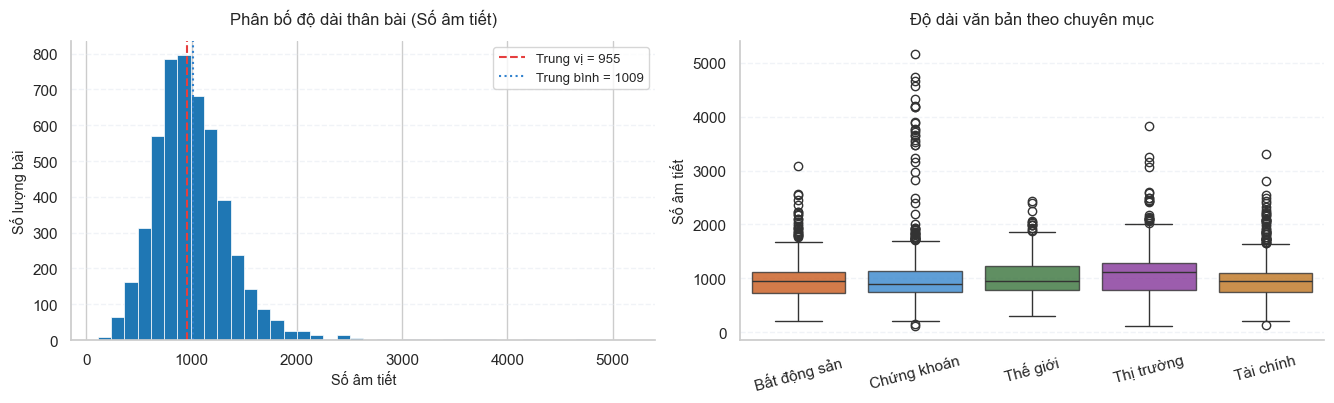
\includegraphics[width=0.86\linewidth]{text/c11_f0.png}
  \caption{Phân phối độ dài bài viết (âm tiết) theo 5 chuyên mục VnEconomy: các chuyên mục có phân phối giao thoa mạnh ($\eta^2 = 0,020$), khẳng định cần dựa vào ngữ nghĩa từ vựng thay vì thống kê độ dài.}
  \label{fig:text_length}
\end{figure}

\begin{figure}[H]
  \centering
  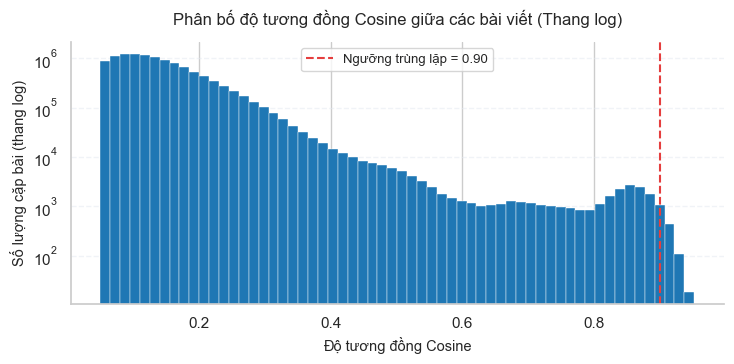
\includegraphics[width=0.86\linewidth]{text/c14_f0.png}
  \caption{Phân tích các cặp bài viết gần trùng (Cosine $\ge 0,90$): phát hiện 18 nhóm (248 bài, 5,0\% tập dữ liệu), là căn cứ để thiết kế phân chia nhóm chống rò rỉ.}
  \label{fig:text_dup}
\end{figure}

\begin{figure}[H]
  \centering
  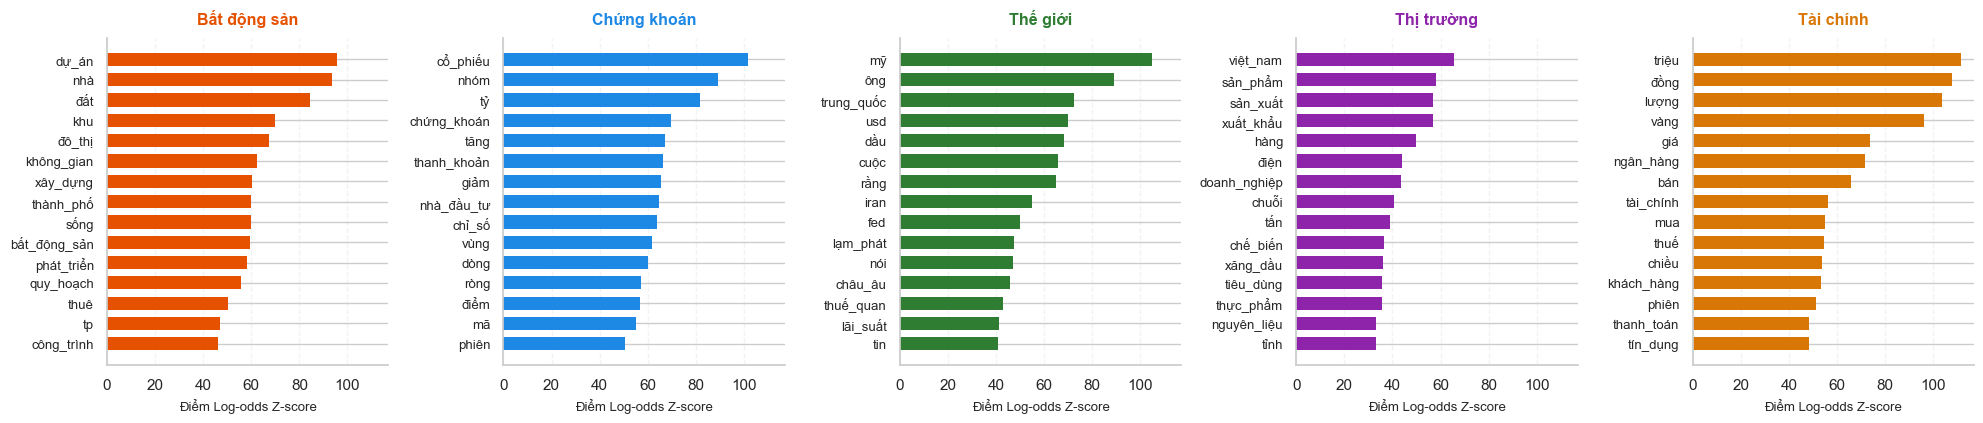
\includegraphics[width=0.88\linewidth]{text/c25_f0.png}
  \caption{Top từ khóa đặc trưng từng chuyên mục theo \textit{Log-odds Z-score}: phản ánh đúng ngữ nghĩa chuyên ngành (ví dụ mã chứng khoán, bất động sản, tỷ giá, địa chính trị).}
  \label{fig:text_keywords}
\end{figure}

\subsection{Thiết kế Pipeline chống rò rỉ và Huấn luyện mô hình}
Để ngăn rò rỉ các bài viết gần trùng, dữ liệu được chia bằng \textbf{StratifiedGroupKFold} theo mã nhóm gần trùng (\texttt{dup\_group}): \textbf{Train/Val} gồm 3.933 bài và \textbf{Test} độc lập gồm 1.067 bài (0 nhóm trùng giữa Train/Val và Test).

Nhóm sử dụng biểu diễn TF-IDF kết hợp tối ưu siêu tham số qua \texttt{GridSearchCV} trên 3 mô hình: \textbf{LinearSVC}, \textbf{Logistic Regression}, và \textbf{Multinomial Naive Bayes}.

\subsection{Kết quả thực nghiệm, Kiểm chứng độ bền và Phân tích lỗi}

\Cref{tab:text_results} và \Cref{fig:text_compare} tổng hợp kết quả đánh giá trên CV và tập Test độc lập (1.067 bài). \textbf{LinearSVC} ($C=100$, n-gram $(1,2)$, bỏ stopword) đạt hiệu năng cao nhất với Test Macro-F1 = \textbf{0,9668} (CI 95\%: $[0,956; 0,977]$), kế đến là Logistic Regression ($0,9603$) và MultinomialNB ($0,9207$). Kiểm định McNemar giữa LinearSVC (1.031/1.067 bài đúng) và Logistic Regression (1.024/1.067 bài đúng) cho $p = 0,118$ (hiệu Macro-F1 $= +0,0066$), cho thấy hai mô hình tuyến tính này tương đương thống kê ở mức $\alpha = 0,05$.

\begin{table}[H]
  \centering
  \caption{Đối chiếu hiệu năng 3 mô hình phân loại văn bản trên Cross-Validation và tập Test độc lập (1.067 bài).}
  \label{tab:text_results}
  \resizebox{\linewidth}{!}{%
  \begin{tabular}{l c c c c}
    \toprule
    \textbf{Mô hình} & \textbf{CV Macro-F1} & \textbf{Test Accuracy} & \textbf{Test Macro-F1} & \textbf{CI 95\% (Test Macro-F1)} \\
    \midrule
    MultinomialNB & $0,9205 \pm 0,0037$ & 0,9203 & 0,9207 & $[0,904;\; 0,936]$ \\
    Logistic Regression & $0,9523 \pm 0,0046$ & 0,9597 & 0,9603 & $[0,949;\; 0,971]$ \\
    LinearSVC & $\mathbf{0,9582 \pm 0,0033}$ & \textbf{0,9663} & \textbf{0,9668} & $\mathbf{[0,956;\; 0,977]}$ \\
    \bottomrule
  \end{tabular}%
  }
\end{table}

\begin{figure}[H]
  \centering
  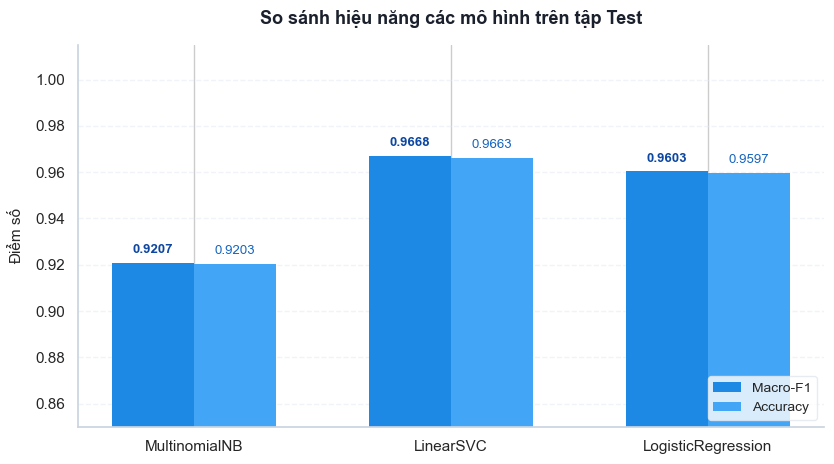
\includegraphics[width=0.86\linewidth]{text/c46_f0.png}
  \caption{So sánh Macro-F1 kèm khoảng tin cậy 95\% trên tập Test (1.067 bài): LinearSVC (0,9668) và Logistic Regression (0,9603) vượt trội rõ rệt so với MultinomialNB (0,9207).}
  \label{fig:text_compare}
\end{figure}

\begin{figure}[H]
  \centering
  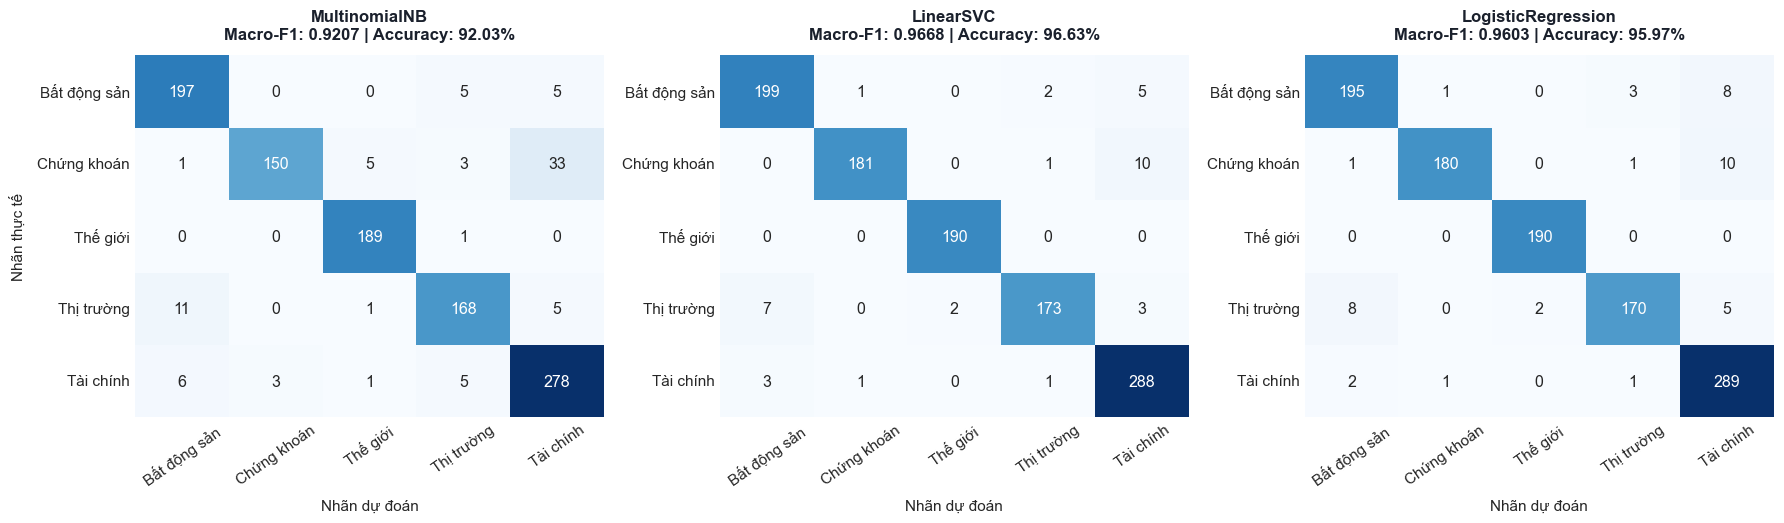
\includegraphics[width=0.82\linewidth]{text/c47_f0.png}
  \caption{Ma trận nhầm lẫn của LinearSVC trên tập Test: lớp \textit{Thế giới} đạt F1 = 0,995; tổng số ca dự đoán sai là 36/1.067 bài, chủ yếu giữa các chuyên mục kinh tế giao thoa như \textit{Tài chính}, \textit{Thị trường} và \textit{Chứng khoán}.}
  \label{fig:text_cm}
\end{figure}

\paragraph{Kiểm chứng độ bền (\textit{Robustness}) và Phân tích lỗi:}
\begin{itemize}[leftmargin=*]
  \item \textbf{Khử trùng hoàn toàn trên Test:} Khi loại bỏ các bài thuộc nhóm gần trùng trên tập Test (còn 939 bài), Macro-F1 của LinearSVC chỉ giảm nhẹ từ $0,9668$ xuống \textbf{0,9611} (Accuracy $= 0,9617$), chứng minh mô hình không học vẹt bản tin lặp.
  \item \textbf{Bóc tách đặc trưng số (\texttt{text\_seg} vs \texttt{text\_num}):} Thay thế số và tỷ lệ phần trăm bằng token đại diện (\texttt{\_so\_}, \texttt{\_pct\_}) giúp CV Macro-F1 tăng nhẹ từ $0,9582 \pm 0,0033$ lên $0,9592 \pm 0,0026$ (giảm phương sai giữa các fold).
  \item \textbf{Kiểm chứng rò rỉ văn phong tác giả (\Cref{fig:text_author}):} Khi chia \texttt{StratifiedGroupKFold} theo \texttt{author\_clean} (đánh giá trên bài của các tác giả chưa từng xuất hiện trong Train), CV Macro-F1 giảm từ $0,9582 \pm 0,0033$ xuống \textbf{0,8519 $\pm$ 0,1030}. Điều này chứng minh một phần hiệu năng cao của mô hình đến từ đặc trưng văn phong riêng của phóng viên chuyên mục.
  \item \textbf{Phân tích 36 ca lỗi trên Test (\Cref{fig:text_cm}):} Có 23 ca nằm ở vùng biên mờ (hiệu điểm top-1 và top-2 $< 0,5$) do giao thoa chủ đề thực sự (ví dụ tin ngân hàng -- chứng khoán -- bất động sản), và 13 ca mô hình tự tin cao ($\ge 0,5$) nhưng gán nhầm nhãn chuyên mục của tòa soạn.
\end{itemize}

\begin{figure}[H]
  \centering
  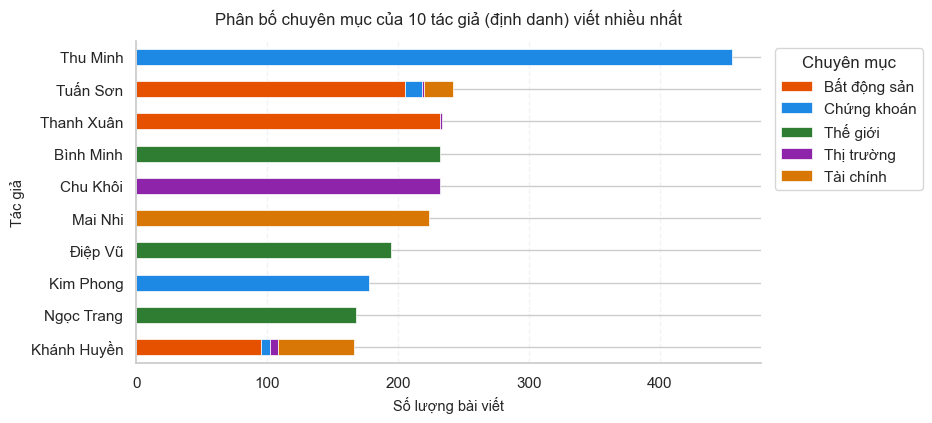
\includegraphics[width=0.84\linewidth]{text/c36_f0.png}
  \caption{Phân bố bài viết theo tác giả: 10 tác giả viết nhiều nhất chiếm 46,5\% tổng số bài, giải thích vì sao chỉ dùng tên tác giả đã đoán đúng 92,3\% chuyên mục và làm CV giảm xuống 0,8519 khi chia tách theo tác giả.}
  \label{fig:text_author}
\end{figure}
